\chapter{Desenvolvimento}
O processo de desenvolvimento englobou, através de uma metodologia definida, a associação do que deveria ser elaborado para que se fosse possível alcançar os objetivos propostos.

É detalhado primeiramente o ambiente de simulação a qual a aplicação utilizou como base, escapando de problemas habituais pré programados propondo uma questão personalização e palpável, assim podendo não apenas alcançar resultados numéricos mas também sendo possível enxergar a sua influência através de uma interface gráfica amigável.

Por fim, se faz a exposição do algoritmo NEAT utilizado como base e seu passo a passo de funcionamento, detalhando a disposição de seus dados, suas estruturas de decisão, impactos da parametrização, evidenciação de resultados e etapas as quais se faz possível realizar um paralelo com redes neurais e algoritmos genéticos.

\section{Metodologia}

O processo de desenvolvimento englobou, através de uma metodologia definida, a associação do que deveria ser elaborado para que se fosse possível alcançar os objetivos propostos.

É detalhado primeiramente o ambiente de simulação a qual a aplicação utilizou como base, escapando de problemas habituais pré programados propondo uma questão personalização e palpável, assim podendo não apenas alcançar resultados numéricos mas também sendo possível enxergar a sua influência através de uma interface gráfica amigável.

Por fim, se faz a exposição do algoritmo NEAT utilizado como base e seu passo a passo de funcionamento, detalhando a disposição de seus dados, suas estruturas de decisão, impactos da parametrização, evidenciação de resultados e etapas as quais se faz possível realizar um paralelo com redes neurais e algoritmos genéticos.

\section{Simula{\c c}{\~a}o}

O objetivo proposto implica no treinamento de carros autônomos
que pudessem vir a ser dispostos em ambientes práticos de modo
a saber lidar com seus arredores e alcançar resultados
práticos. Seja o ambiente real uma réplica do circuito
presente na aplicação ou um ambiente novo, a validação dos
testes vem a acontecer em sua totalidade através de um
\textit{software} desenvolvido.

Este espaço virtual visa simular um carro dentro de um
circuito fechado cercado por paredes, o qual, pondo em prática
sua autonomia, está equipado de sensores que medem sua
distância ao bloqueio mais próximo à sua frente, e num
intervalo de 45° para ambos os lados até se tornarem
perpendiculares, somando-se assim cinco distâncias a serem
medidas. Na \autoref{fig_simul} pode-se observar a representa{\c c}{\~a}o gr{\'a}fica desse espa{\c c}o.

\begin{figure}[htb]
        \centering
        \caption{\label{fig_simul}Interface gráfica utilizada para a simulação, com o modelo de carro autônomo, trajeto de treino a ser percorrido e botões de controle de \textit{layout}.}
        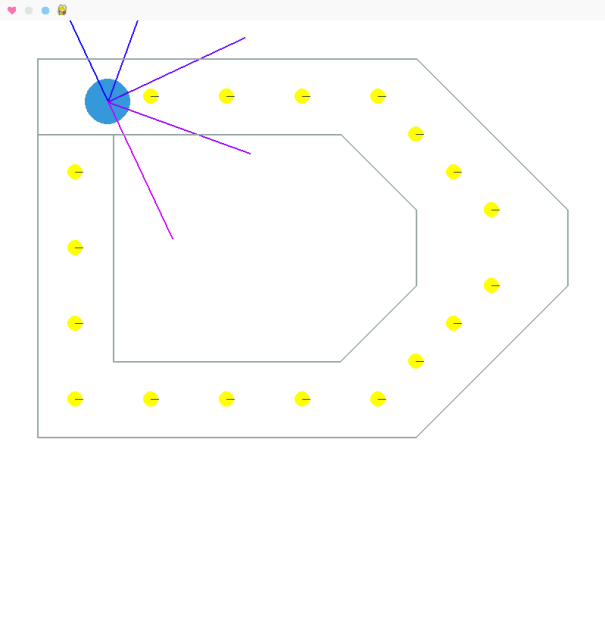
\includegraphics[width=0.7\textwidth]{images/simul.png}
        \legend{
                Fonte: Autoria Pr{\'o}pria.
        }
\end{figure}

O ambiente de simulação utilizado como base para os
experimentos foi desenvolvido em python com a biblioteca
\textit{pygame}, sua interface oferece métodos baseando-se em
orientação a objeto para a elaboração de jogos e aplicações
multimídia, através desta se fez o design da janela de
execução com seus elementos de tela (botões e limites do
circuito). Em conjunto, se faz uso da biblioteca de física 2d
\textit{pymunk}, para controlar a movimentação e colisão do carro.

A configuração do carro, no que diz respeito à sua interação
com ambiente, engloba:

\begin{enumerate}
	\item A posição inicial do carro e a distância por ele percorrida, utilizadas posteriormente como indicadores de desempenho para o algoritmo de neuroevolução;
	\item A forma do carro, a princípio definida como um círculo para facilitar sua movimentação pelo espaço, evitando colisões involuntárias;
	\item Sensoriamento do carro, identificando sua distância às paredes, posteriormente sendo utilizado para tomadas de decisão.
\end{enumerate}


\section{APLICA{\c C}{\~A}O DO ALGORITMO NEAT}
A sequência de execução a qual o algoritmo está sujeito pode ser expressa na \autoref{fig_flowchart}, o fluxograma idealiza a ordem dos fatores que vão desde a criação dos carros que compõem uma população, às suas tomadas de decisão e avaliações, passando pelo processo de reprodução, mutação e especiação das redes neurais que os compõem, até finalmente o ciclo se reiniciar ou seu encerramento ser julgado adequado.

\begin{figure}[htb]
        \centering
        \caption{\label{fig_flowchart}Fluxograma geral de execução do algoritmo NEAT aplicado à simulação.}
        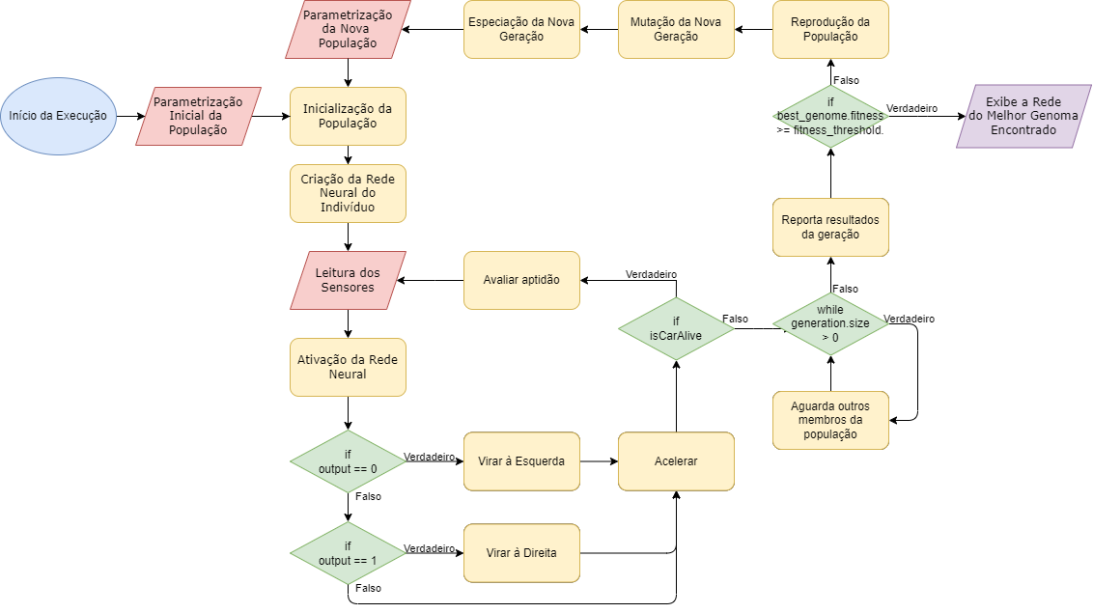
\includegraphics[width=0.7\textwidth]{images/flowchart.png}
        \legend{
                Fonte: Autoria Pr{\'o}pria.
        }
\end{figure}

\subsection{Início Pré Execução}
A etapa inicial da execução do algoritmo contempla a criação dos membros da população e a forma pela qual os parâmetros predefinidos devem redigir suas ações. Estas propriedades vêm a ditar suas duas principais componentes, o genoma, da parte constituinte do algoritmo genético e a rede neural, da parcela de aprendizado de máquina.

\subsubsection{Parametrização Predefinida Inicial}
De maneira prévia à execução, se faz necessária a atribuição de parâmetros que virão a ser utilizados pelo algoritmo para controlar seu processo evolucionário. Estes dados são geralmente ajustados em meio a execuções a fins de se obter resultados mais próximos dos ideais.

A sensibilidade do algoritmo genético o permite ser implementado de diferentes formas, tal qual apontado por PACHECO (1999), “A escolha de técnicas, parâmetros e tipos de operadores é empírica, porém em sintonia com o problema.”, expondo a necessidade de empregar a melhor abordagem ao problema em questão não sendo ela uma verdade universalmente aplicável.

Desta forma, ao algoritmo proposto à simulação desenvolvida, os parâmetros podem ser divididos em subgrupos que atingem diferentes partes do ciclo de execução. Suas definições gerais de funcionamento e reprodução podem ser exemplificadas na \autoref{fig_CA}.

\begin{figure}[htb]
        \centering
        \caption{\label{fig_CA}Parametrizações gerais e de reprodução.}
        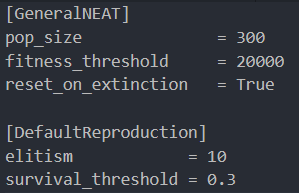
\includegraphics[width=0.7\textwidth]{images/CA.png}
        \legend{
                Fonte: Autoria Pr{\'o}pria.
        }
\end{figure}

Primeiramente, o tamanho da população corresponde à quantidade de carros concorrentes a cada geração. O limite mínimo de aptidão define, em eventual obtenção de tal valor de aptidão por qualquer membro da geração, que a simulação se encerre e seja dada a rede encontrada como resposta obtida.

Quanto à sua reprodução, a propriedade de elitismo define quantos membros de uma geração encerrada devem seguir como cópias à geração seguinte, enquanto o limite de sobrevivência é responsável por limitar a porcentagem de membros de uma geração encerrada que devem se incumbir da tarefa de se reproduzir e gerar a próxima geração.

Quanto às definições específicas aos genomas e suas interações passíveis a alterações de topologia, é possível observar as configurações iniciais na \autoref{fig_CB}, a maneira da qual cada parâmetro afeta o desempenho do algoritmo será abordada detalhadamente em capítulos posteriores.

\begin{figure}[htb]
        \centering
        \caption{\label{fig_CB}Parametrizações de genomas e redes neurais.}
        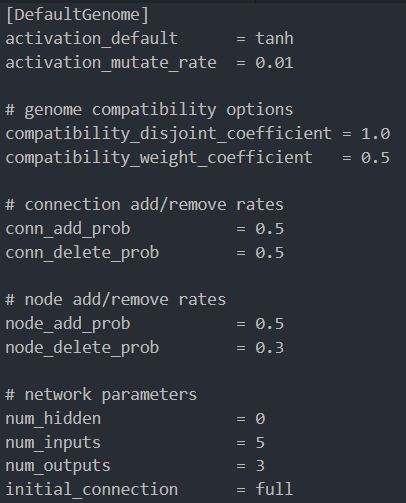
\includegraphics[width=0.7\textwidth]{images/CB.png}
        \legend{
                Fonte: Autoria Pr{\'o}pria.
        }
\end{figure}

A função de ativação de cada nó da rede pode ser definida tal qual a sua probabilidade de sofrer uma mutação — decorrendo-se na etapa adequada de reprodução. A compatibilidade de nós define qual similares dois nós devem ser para que seu processo de crossover seja possível considerando ambos como portadores da mesma informação genética.

Efetivamente, a modificação de topologias — que oferece o nome ao algoritmo de Topologias Aumentantes — acontece em razão das probabilidades definidas para adição ou remoção de conexões ou nós da camada oculta, resultando em uma alteração de seu formato a uma forma possivelmente ideal para aquele indivíduo que vier a sofrer a mutação.

Por fim, os parâmetros básicos da rede definem sua forma inicial, sendo sempre tratada como cinco entradas (sensoriamento), três saídas (direções a serem tomadas), com total conexão entre nós, e zero camadas ocultas. Esta última se dá pelo princípio apresentado no Capítulo 4.3 o qual reforça a prática de partir de uma estrutura mínima pois a inicialização de uma rede neural densa pode vir a ser muito custosa e o algoritmo precisaria de muito tempo para otimizar estruturas complexas \cite{stanley2004neat}. Sua estrutura inicial pode ser representada pela \autoref{fig_CC}.

\begin{figure}[htb]
        \centering
        \caption{\label{fig_CC}Organização inicial da rede neural partindo de uma estrutura mínima.}
        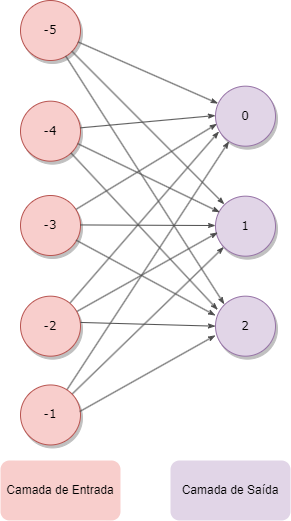
\includegraphics[width=0.7\textwidth]{images/CC.png}
        \legend{
                Fonte: Autoria Pr{\'o}pria.
        }
\end{figure}

\subsubsection{Inicialização da População}
Considerando a arquitetura de Neuroevolução de Topologias Aumentantes como uma junção das esferas de Algoritmos Genéticos e Redes Neurais, a grande maioria de seus conceitos básicos também são expressos na construção desta mescla.

Partindo deste princípio, a \autoref{fig_DA} ilustra a construção básica da qual são englobados todos os membros da população da simulação, exemplificados como carros. Os dois principais componentes podem ser expressos como:

\begin{enumerate}
	\item \textit{genome} — cromossomo com as características do carro — Composto pelas propriedades que diferenciam cada membro da população, como o peso em suas arestas de conexão, fitness e nós totais, e também as propriedades que acatam todos os indivíduos da mesma população, como as chances de ganhar ou perder nós ou conexões durante a mutação, além da probabilidade deste processo ocorrer e a estrutura inicial a ser passada para a rede no momento de sua criação; 
	\item \text{brain} —  rede a qual este carro está sujeito — sendo esta composta por todo o seu conjunto de entradas, nós da camada oculta e de saída. Também é responsável pelo processo de tomada de decisão, baseando-se na rede criada a partir das conexões provindas do genoma de origem, retornando uma saída interpretada adequada.
\end{enumerate}

\begin{figure}[htb]
        \centering
        \caption{\label{fig_DA}Propriedades básicas do algoritmo NEAT pertencentes a cada membro da população.}
        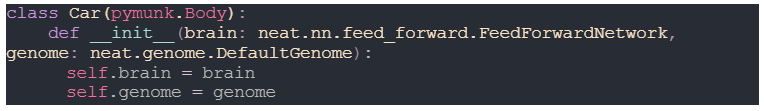
\includegraphics[width=0.7\textwidth]{images/DA.png}
        \legend{
                Fonte: Autoria Pr{\'o}pria.
        }
\end{figure}

\subsubsection{Criação da Rede Neural Individual}
Cada indivíduo da população parte de um mesmo genótipo — levando em conta o princípio de estruturas iniciais mínimas — este (tratado como genoma) carrega informações referentes aos nós que o compõem e as suas conexões, cada qual com seu devido viés que influenciará nas etapas futuras a tomada de decisão e a especiação de cada membro.

A fins de implementação, as entradas da rede não são interpretadas como nós, por estas não poderem possuir viés atrelado aos valores lidos pelo sensoriamento dos carros. Os demais nós são definidos por três componentes: 

\begin{enumerate}
	\item Identificador, com a intenção de diferenciar o genoma originário que compõe a rede de cada indivíduo da população;
	\item Viés, constante aplicável à função de ativação com a intenção de movê-la, influenciando no resultado de saída (tomada de decisão);
	\item Função de ativação, responsável por definir a saída de um nó dado valores de entrada.
\end{enumerate}

As conexões presentes em cada genoma — interpretáveis como genes — definem quais nós se encontram interconectados na rede neural de determinado indivíduo, o viés aplicável a suas arestas e seu status de ativação (relevante para o processo de reprodução.

Uma forma de representar o genoma de determinado indivíduo de exemplo é observável na \autoref{fig_EA}, onde as conexões foram resumidas para a representação gráfica.

\begin{figure}[htb]
        \centering
        \caption{\label{fig_EA}Exemplo de genoma empregado com os respectivos nós, conexões e seus vieses.}
        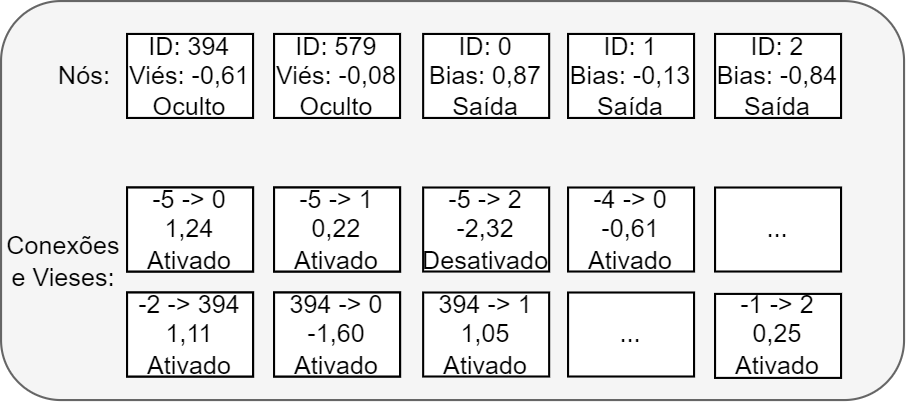
\includegraphics[width=0.7\textwidth]{images/EA.png}
        \legend{
                Fonte: Autoria Pr{\'o}pria.
        }
\end{figure}

Partindo de um genoma, a criação da rede se fundamenta em unir os nós de acordo com as conexões estabelecidas, o trecho de código da \autoref{fig_EB} demonstra como a implementação foi realizada. A visualização da rede básica criada pode ser vista na \autoref{fig_CC}, traçando um paralelo como um Algoritmos Genéticos, a representação gráfica de um genótipo é observável como um fenótipo, no caso, a visualização da rede.

\begin{figure}[htb]
        \centering
        \caption{\label{fig_EB}Criação de rede neural individual a partir de um genoma de origem.}
        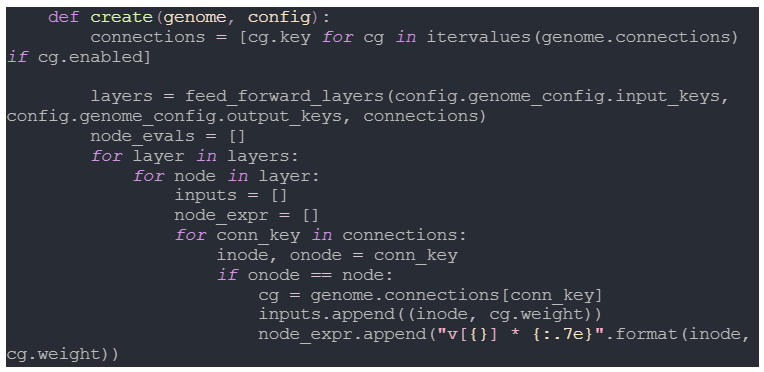
\includegraphics[width=0.7\textwidth]{images/EB.png}
        \legend{
                Fonte: Autoria Pr{\'o}pria.
        }
\end{figure}

A rede neural desenvolvida se trata de uma Rede Neural Feed-forward, de acordo com \citeonline{montana1989davis}, definida por possuir topologia sem caminhos fechados , ou seja, é impossível um nó retornar à camada anterior de modo a executar um loop, o que a tornaria recorrente. 

Esta rede também não está sendo feita com o conceito de backpropagation implementado, considerando que este cenário de testes não possui dados de treino para basear seu desempenho além da própria aptidão obtida, comparável apenas dentro da própria população. Isso acarreta na alteração de peso das arestas ocorrendo exclusivamente pelo processo de reprodução.

\subsection{Processo de Execução}
A etapa seguinte da execução do algoritmo trata do fluxo individual de cada carro após a sua parametrização e inicialização. Abrangendo a entrada de dados do ambiente de simulação ao carro, e a maneira a qual ele as interpreta e toma decisões em relação a que direção seguir, culminando em um aumento de fitness e posterior avaliação.

\subsubsection{Leitura do Ambiente}
A \autoref{fig_GA} exibe os métodos implementados responsáveis por identificar a distância do carro em relação aos obstáculos do ambiente, de modo a atualizá-la em caso de alteração e recuperação para leitura. Estes valores são armazenados como números de ponto flutuante.

\begin{figure}[htb]
        \centering
        \caption{\label{fig_GA}Sensoriamento do carro para obtenção de distâncias em relação ao ambiente.}
        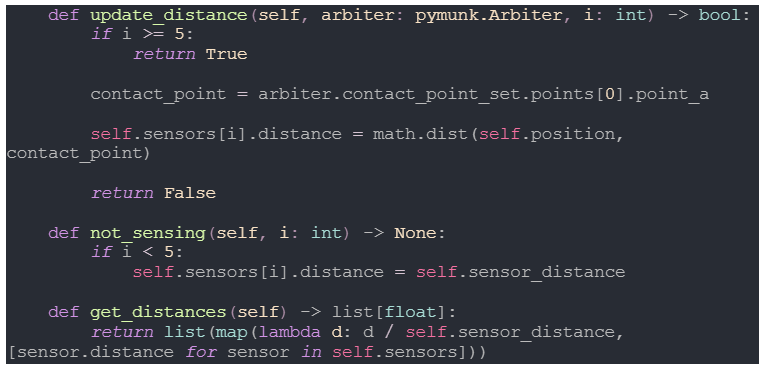
\includegraphics[width=0.7\textwidth]{images/GA.png}
        \legend{
                Fonte: Autoria Pr{\'o}pria.
        }
\end{figure}

De modo a exemplificar uma leitura de dados, a \autoref{fig_GB} representa um carro com os sensores à direita e frente próximos à parede enquanto os sensores à esquerda percorrem uma distância maior até encontrarem a parede, ou sequer a encontram.

\begin{figure}[htb]
        \centering
        \caption{\label{fig_GB}Exemplo de sensores à direita e frente próximos aos limites do circuito e à esquerda livres.}
        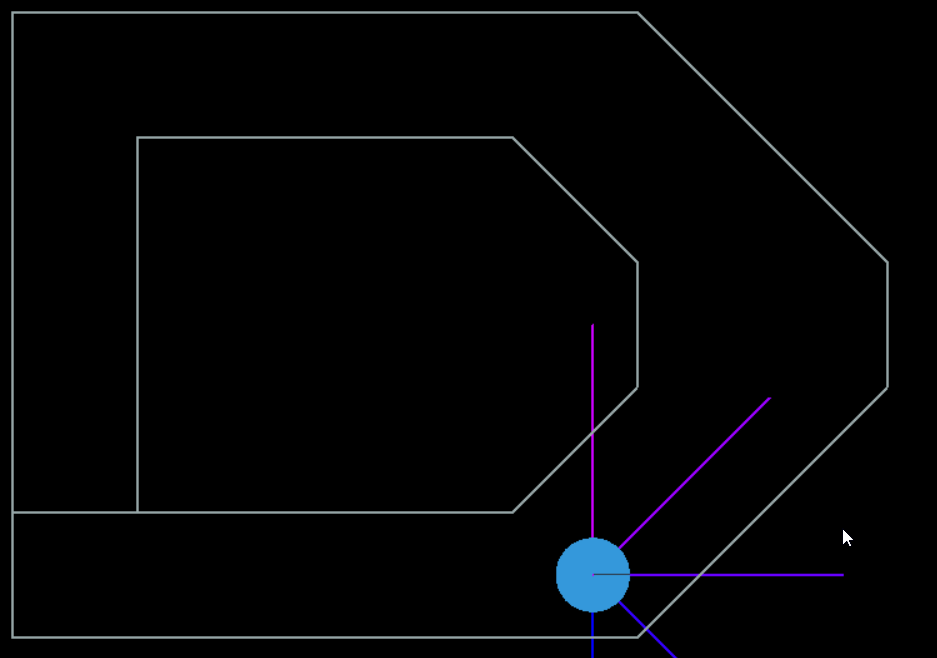
\includegraphics[width=0.7\textwidth]{images/GB.png}
        \legend{
                Fonte: Autoria Pr{\'o}pria.
        }
\end{figure}

Através da Tabela GZ é possível estimar valores lidos para este instante, os sensores seguem a ordem numérica de identificadores -5 a -1 considerando o sentido horário da Figura GB, sendo -5 o sensor mais à esquerda e -1 o mais à direita da perspectiva do veículo. Também é possível observar na \autoref{tab_GZ} os pesos obtidos entre as conexões de cada sensor com cada uma das saídas n após o final da execução, considerando esta uma topologia simples de cinco entradas e três saídas totalmente interconectadas.

\begin{table}[htb]
	\centering
    \caption{\label{tab_GZ}Valores lidos individualmente lidos pelos sensores com o peso de suas arestas às saídas.}
    \begin{tabular}{ccccc}
        \hline
		\textbf{Sensores} & \textbf{Entradas (px)} & \textbf{Peso Con. n0} & \textbf{Peso Con. n1} & \textbf{Peso Con. n2} \\ \hline
		-5 & 120  & 0,057   & 0,740  & 1,656   \\ \hline
		-4 & 200  & 2,588   & -1,330  & -2,810   \\ \hline
		-3 & 50  & -1,178   & 0,063  & 1,559   \\ \hline
		-2 & 30  & -1,783   & 0,318  & 1,172  \\ \hline
		-1 & 10  & -1,007   & -1,469  & -0,238   \\ \hline
    \end{tabular}
    \fonte{Autoria pr{\'o}pria.}
\end{table}

\subsubsection{Ativação da Rede Neural}
Os valores lidos a cada frame são coletados e enviados como parâmetros para a função de ativação da rede neural (vide \autoref{fig_HA}), esta vem a retornar um vetor de saídas, o qual indica qual das saídas deve vir a ser ativada para a tomada de decisão do carro.

\begin{figure}[htb]
        \centering
        \caption{\label{fig_HA}Chamada do método de ativação da rede neural baseando-se nos valores lidos.}
        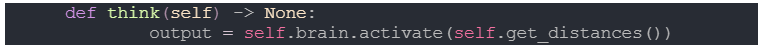
\includegraphics[width=0.7\textwidth]{images/HA.png}
        \legend{
                Fonte: Autoria Pr{\'o}pria.
        }
\end{figure}

Após recebidos os valores das cinco entradas, o método de ativação as utiliza multiplicando suas leituras pelo peso de cada uma de suas três arestas, observável na \autoref{tab_HZ}.

\begin{table}[htb]
	\centering
    \caption{\label{tab_HZ}Produto entre a leitura dos sensores e o peso de cada uma de suas arestas.}
    \begin{tabular}{ccccc}
        \hline
		\textbf{Sensores} & \textbf{Entrada * w$_{\text{1i}}$} & \textbf{Entrada * w$_{\text{2i}}$} & \textbf{Entrada * w$_{\text{3i}}$} \\ \hline
		-5 & 6,840  & 88,800   & 198,720    \\ \hline
		-4 & 517,600  & -266,000   & -562,000    \\ \hline
		-3 & -58,900  & 3,150   & 77,950   \\ \hline
		-2 & -53,490  & 9,540   & 35,160  \\ \hline
		-1 & -10,070  & -14,690   & -2,380   \\ \hline
    \end{tabular}
    
    \fonte{Autoria pr{\'o}pria.}
\end{table}

O produto resultante vem a ser utilizado para a função agregada aplicada aos nós – definida como somatório de início da execução, podendo vir a sofrer mutação, desconsiderada para fins de demonstração padronizada. 

O valor é obtido somando todas as entradas pesadas com as arestas para cada saída, podendo ser observado na \autoref{images/tab_HY}.

\begin{table}[htb]
	\centering
    \caption{\label{tab_HY}Resultados da função agregada de somatório das arestas pesadas às entradas para cada nó de saída.}
    \begin{tabular}{ccccc}
        \hline
		\textbf{Sa\'{i}das} & \textbf{Fun\c{c}\~{a}o Agregada} \\ \hline
		0 & 401,980    \\ \hline
		1 & -179,200    \\ \hline
		2 & -252,550  \\ \hline
    \end{tabular}
    
    \fonte{Autoria pr{\'o}pria.}
\end{table}

A resposta da função agregada é utilizada como variável independente para a função polinomial de primeiro grau a ser utilizada como entrada à função de ativação. A \autoref{tab_HX} ilustra o resultado obtido para cada variável dependente \textit{f(x)}  seguindo a equação aplicável a cada saída n.

\[ f(x) = bias + response * agg_func(n)\]

O parâmetro \textit{bias} (viés de cada nó) assume o papel de constante da função realizando o ajuste adequado à resposta, este se soma ao resultado da função agregada multiplicado pela \textit{response} (resposta) recebida do nó anterior, por tratar-se da camada de entrada da rede neural, este é interpretado como 1 (um) de modo a não influenciar o restante da equação.

\begin{table}[htb]
	\centering
    \caption{\label{tab_HX}Resultados da função polinomial de primeiro grau aplicados a cada nó de saída levando em consideração seu viés e resposta oriunda da camada anterior.}
    \begin{tabular}{ccccc}
        \hline
		\textbf{Sa\'{i}das} & \textbf{Fun\c{c}\~{a}o Polinomial} \\ \hline
		0 & 403,758    \\ \hline
		1 & -179,536    \\ \hline
		2 & -250,866  \\ \hline
    \end{tabular}
    
    \fonte{Autoria pr{\'o}pria.}
\end{table}

Finalmente, o resultado da função polinomial pode ser aplicado à função de ativação de cada nó – definida como tangente hiperbólica \textit{tanh(z)} ao início da execução, esta pode vir a sofrer mutação após o processo de reprodução, porém o cenário foi desconsiderado para padronizar a demonstração.

A função empregada assume fórmula a seguir, onde seu \textit{z} é substituído pelo próprio resultado da função polinomial de primeiro grau.

\[ \sigma(z) = \frac{e^z - e^{-z}}{e^z + e^{-z}}\]

Aplicando a função a cada uma das saídas, obtém-se os resultados presentes na \autoref{tab_HW}, onde seus valores de saída estão arredondados para 1 ou -1 considerando a escala imensa e trivial para a resolução do problema.

\begin{table}[htb]
	\centering
    \caption{\label{tab_HW}Resultados da função de ativação de tangente hiperbólica a cada nó de saída.}
    \begin{tabular}{ccccc}
        \hline
		\textbf{Sa\'{i}das} & \textbf{Fun\c{c}\~{a}o de Ativa\c{c}\~{a}o} \\ \hline
		0 & 1    \\ \hline
		1 & -1    \\ \hline
		2 & -1  \\ \hline
    \end{tabular}
    
    \fonte{Autoria pr{\'o}pria.}
\end{table}

O resultado obtido identifica a saída 0 como contendo o maior valor retornado da função de ativação – sem a necessidade de desconsiderar o arredondamento, no caso.

O trecho de código com a implementação do cálculo de saída pode ser observado na \autoref{fig_HM}.

\begin{figure}[htb]
        \centering
        \caption{\label{fig_HM}Implementação do método de ativação da rede neural baseando-se nos valores lidos, retornando o valor de ativação de cada nó de saída.}
        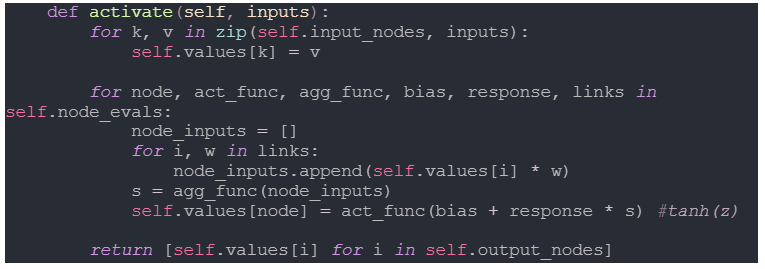
\includegraphics[width=0.7\textwidth]{images/HM.png}
        \legend{
                Fonte: Autoria Pr{\'o}pria.
        }
\end{figure}

\subsubsection{Tomada de Decisão}
Considerando o retorno da função como a lista de ativações dos nós de saída, se faz necessário filtrar apenas o valor de maior expressão numérica, como concretizado na \autoref{fig_HN}.

Sua estrutura de decisão seguinte implica na tomada de decisão visível do carro, onde ele se angula à esquerda em caso de saída equivalente a 0, à direita ao retorno de 1 e segue em frente sem alterações de direção em caso de ativação do nó de número 2.

\begin{figure}[htb]
        \centering
        \caption{\label{fig_HN}Retorno do maior valor de ativação dos nós de saída e tomada de decisão.}
        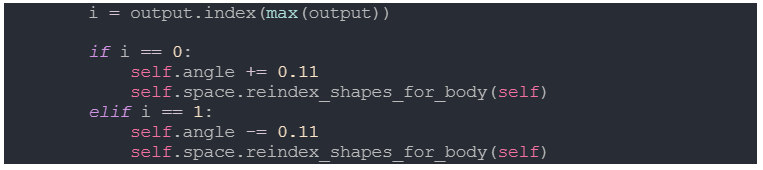
\includegraphics[width=0.7\textwidth]{images/HN.png}
        \legend{
                Fonte: Autoria Pr{\'o}pria.
        }
\end{figure}

A função completa com todas as etapas anteriores pode ser expressa pela seguinte fórmula:

\[ output = \max_{n}\{n | tanh(bias + response * \sum_{k=0}^{\i} weight_{ni}*input)\} \]

Retornando à situação proposta na Figura GB e minuciosamente examinada no subcapítulo 5.3.2.2, se faz possível notar uma tendência a virar à esquerda de acordo com o ambiente sensorizado – ativação do nó de saída de identificador 0 – onde esta parece ser a alternativa que o manterá vivo por mais tempo.

\subsubsection{Avaliação de Desempenho Individual}
De acordo com o progresso executado pelo carro ao se mover pelo percurso, este contabiliza a distância desde o ponto de partida e a soma em um contador, baseando-se na posição atual e na posição do frame anterior. A \autoref{fig_IA} representa sua implementação através do código 

\begin{figure}[htb]
        \centering
        \caption{\label{fig_IA}Implementação de métodos de recompensa aos carros de acordo com sua distância percorrida.}
        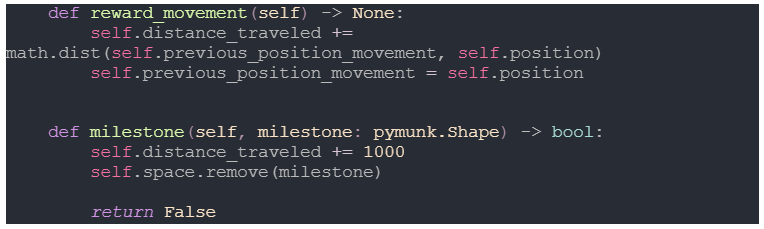
\includegraphics[width=0.7\textwidth]{images/IA.png}
        \legend{
                Fonte: Autoria Pr{\'o}pria.
        }
\end{figure}

Também é possível recompensar o carro com a obtenção de marcos dispostos pelo circuito (círculos amarelos na \autoref{fig_IB}). 

Sua implementação visa acelerar o treinamento dos indivíduos a moverem-se de forma ordenada com o formato da pista, mas sem obrigá-los, considerando que o valor posteriormente atrelado à aptidão não provém exclusivamente desta fonte e a sua não obtenção – ao realizar uma travessia por caminhos levemente alternativos – pode vir a ser uma característica de interesse nas etapas seguintes de reprodução.

\begin{figure}[htb]
        \centering
        \caption{\label{fig_IB}Marcos dispostos pelo circuito a fim de recompensar o movimento ordenado do carro.}
        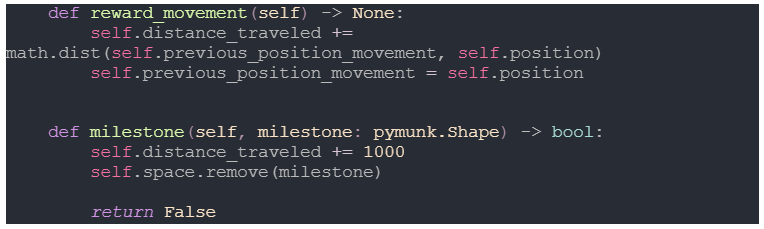
\includegraphics[width=0.7\textwidth]{images/IB.png}
        \legend{
                Fonte: Autoria Pr{\'o}pria.
        }
\end{figure}

A atribuição do valor percorrido à aptidão do genoma presente no carro acontece apenas em sua exclusão do ambiente – proveniente da colisão com o ambiente – efetivando o ciclo de um carro e permitindo que o desempenho atrelado à sua topologia de rede seja reportado para a formulação da nova geração. O encerramento de um indivíduo está apresentado na \autoref{fig_IC}.

\begin{figure}[htb]
        \centering
        \caption{\label{fig_IC}Atribuição de aptidão de acordo com a distância percorrida pelo indivíduo e sua remoção do ambiente visual de simulação.}
        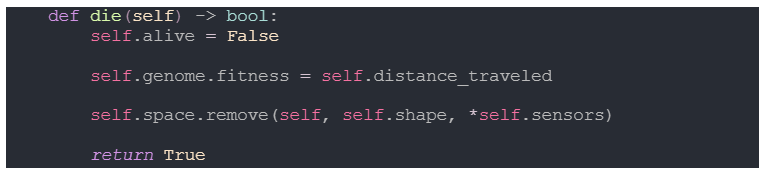
\includegraphics[width=0.7\textwidth]{images/IC.png}
        \legend{
                Fonte: Autoria Pr{\'o}pria.
        }
\end{figure}

\subsection{Avaliação Populacional Pós Execução}
A etapa final do ciclo de execução acontece no momento em que a população se encontra extinta.

A tomada de decisão responsável por verificar se o valor limite de aptidão mínima foi encontrado define se o algoritmo será interrompido e o genoma originário da rede de solução será ou  retornado ou se é necessária a execução de pelo menos mais um ciclo. Os subcapítulos seguintes retratam o cenário em caso de demanda da realização de criação de uma nova geração para a próxima iteração.

\subsubsection{Seleção da População}
Antes do processo de \textit{crossing-over} ser executado, o parâmetro de inicialização \textit{elitism} atua filtrando os melhores indivíduos de cada espécie, criando cópias suas à nova geração e assim mantendo a variabilidade genética da população. A \autoref{fig_KA} apresenta a implementação desta função.

\begin{figure}[htb]
        \centering
        \caption{\label{fig_KA}Aplicação de elitismo sobre cada espécie, preservando os melhores indivíduos de cada espécie à nova geração.}
        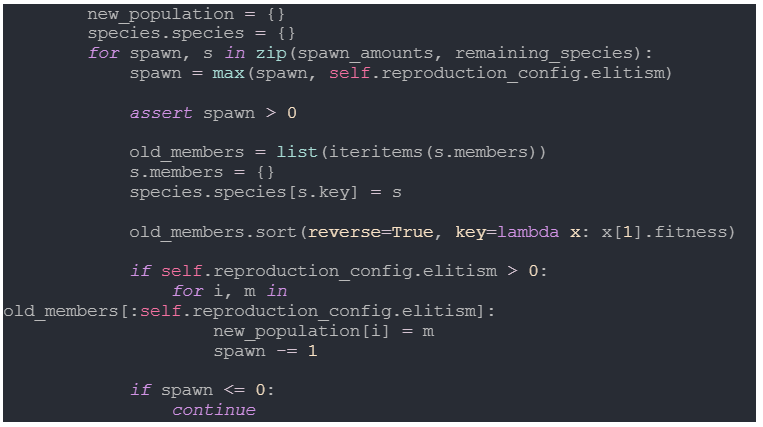
\includegraphics[width=0.7\textwidth]{images/KA.png}
        \legend{
                Fonte: Autoria Pr{\'o}pria.
        }
\end{figure}

O critério para a seleção de membros da população que serão considerados candidatos a pais da próxima geração se baseia em seu desempenho.

Assim como o elitismo define quais membros serão copiados à próxima geração, o limite de sobrevivência – parâmetro de inicialização – define a porcentagem da população a realizar o cruzamento entre si, de modo que a próxima geração seja composta apenas da porcentagem de melhor desempenho da população anterior. Ilustrado na \autoref{fig_KB}.

\begin{figure}[htb]
        \centering
        \caption{\label{fig_KB}Corte da população de melhor aptidão selecionado para a reprodução.}
        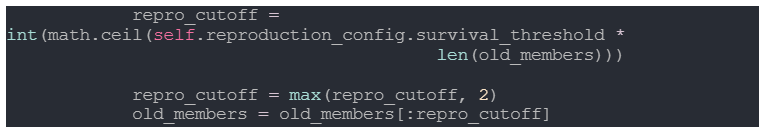
\includegraphics[width=0.7\textwidth]{images/KB.png}
        \legend{
                Fonte: Autoria Pr{\'o}pria.
        }
\end{figure}

Após o processo de seleção, se faz possível iniciar a reprodução através de \textit{crossover} e a mutação dos indivíduos resultantes. A nova população gerada é retornada para ser posteriormente atribuída como a nova geração, como apresenta a \autoref{fig_KC}.

\begin{figure}[htb]
        \centering
        \caption{\label{fig_KC}Chamada do processo de reprodução entre pais aleatórios selecionados e mutação dos filhos resultantes.}
        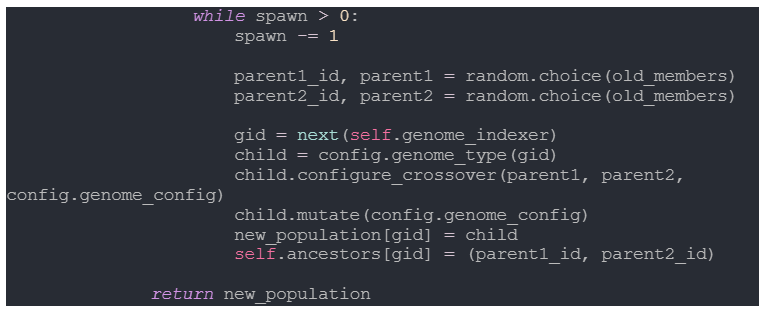
\includegraphics[width=0.7\textwidth]{images/KC.png}
        \legend{
                Fonte: Autoria Pr{\'o}pria.
        }
\end{figure}

\subsubsection{Reprodução da População Selecionada}

O processo de \textit{crossover} se baseia em mesclar o genoma de ambos os pais, seja suas conexões com os devidos pesos ou os nós que compõem as suas camadas com seus devidos vieses.

A \autoref{fig_LA} ilustra o processo de crossover a gerar as conexões do filho. Sua lógica se baseia em comparar qual dos pais possui uma aptidão maior para a tomada de decisão caso os genes sejam disjuntos, isto é, uma informação presente em um dos pais não se encontra no outro.

\begin{figure}[htb]
        \centering
        \caption{\label{fig_LA}\textit{Crossover} entre pais para a geração das conexões de um novo filho.}
        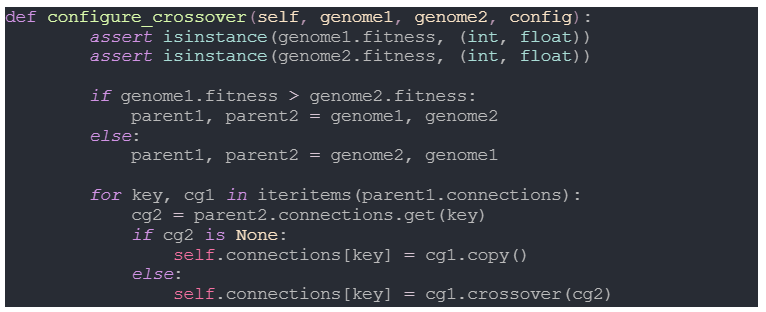
\includegraphics[width=0.7\textwidth]{images/LA.png}
        \legend{
                Fonte: Autoria Pr{\'o}pria.
        }
\end{figure}

Seguindo a mesma lógica do crossover entre conexões, o crossover entre nós também realiza uma verificação da presença de determinado gene entre ambos os pais antes de realizar o cruzamento de fato, sua implementação é observável na \autoref{fig_LB}.

\begin{enumerate}
	\item Em caso de existência de genes disjuntos, este vem a ser atribuído ao filho apenas caso sua presença venha a  ser observada no pai de maior aptidão;
	\item Em caso de genes homólogos, se faz a realização de um crossover entre os genes para sua atribuição ao filho.
\end{enumerate}

\begin{figure}[htb]
        \centering
        \caption{\label{fig_LB}\textit{Crossover} entre pais para a geração dos nós de um novo filho.}
        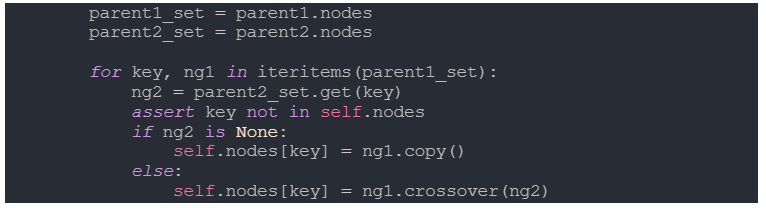
\includegraphics[width=0.7\textwidth]{images/LB.png}
        \legend{
                Fonte: Autoria Pr{\'o}pria.
        }
\end{figure}

\subsubsection{Mutação da Nova Geração}
A etapa de mutação da nova prole acontece logo após sua reprodução estar completa. Nela contemplam a possibilidade de adição ou remoção de nós e conexões, e a alteração de pesos das conexões e viés dos nós.

A \autoref{fig_MA} ilustra a estrutura de decisão a qual cada um dos genomas está sujeito a fim de identificar se sofrerão mutação ou não. Para cada parâmetro entre, remover ou adicionar conexão ou nó, um número aleatório é gerado e caso este se encontre dentro do limite mínimo estabelecido para a condição, este a sofrerá. O trecho de código especifica um cenário de mutação estrutural múltipla, ou seja, cada genoma pode vir a sofrer mais de uma mudança em sua estrutura topológica por processo mutação.

\begin{figure}[htb]
        \centering
        \caption{\label{fig_MA}Estrutura de decisão de mutação aleatória entre filhos recém gerados, considerando uma estrutura sem limite de mutação estrutural múltipla.}
        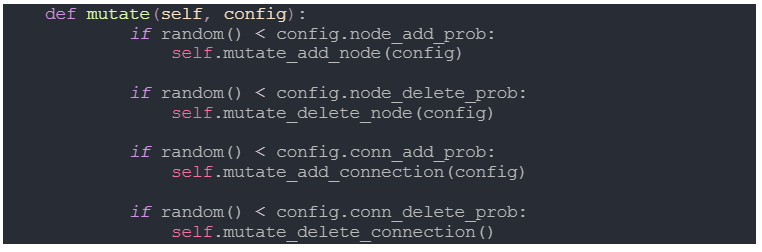
\includegraphics[width=0.7\textwidth]{images/MA.png}
        \legend{
                Fonte: Autoria Pr{\'o}pria.
        }
\end{figure}

Utilizando como exemplo uma adição de nó para a alteração da topologia do filho resultante, a \autoref{fig_MB} ilustra este processo. Uma conexão entre dois nós, ou uma entrada e um nó, se torna desabilitada, enquanto de maneira intermediária um novo nó é criado com as configurações básicas de parametrização definidas fazendo uma ponte entre as antigas entradas e saídas da conexão.

\begin{figure}[htb]
        \centering
        \caption{\label{fig_MB}Implementação da adição de um novo nó ao filho não presente em seus pais através da mutação.}
        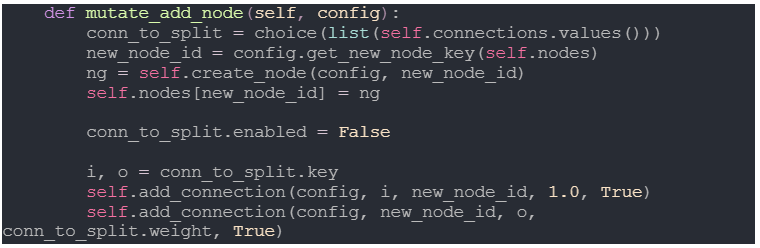
\includegraphics[width=0.7\textwidth]{images/MB.png}
        \legend{
                Fonte: Autoria Pr{\'o}pria.
        }
\end{figure}

A conexão entre o novo nó e antiga entrada assume o peso da antiga conexão, enquanto a conexão entre o novo nó e a antiga saída assume um peso predefinido de uma (1) unidade. A \autoref{fig_MC} ilustra a antiga conexão ao topo e a nova conexão na parte inferior, utilizando-se de uma entrada -5 e um nó de saída 0 como exemplos.

\begin{figure}[htb]
        \centering
        \caption{\label{fig_MC}Exemplo de mutação entre uma entrada e uma saída recebendo um novo nó intermediário, alterando a topologia resultante.}
        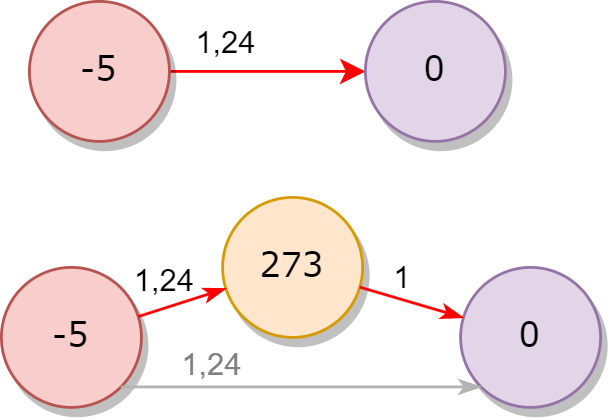
\includegraphics[width=0.7\textwidth]{images/MC.png}
        \legend{
                Fonte: Autoria Pr{\'o}pria.
        }
\end{figure}

\subsubsection{Especiação da Nova Geração}
Com a intenção de valorizar a inovação dentre as informações contidas em uma população, é de sumo interesse que indivíduos que alcancem resultados aceitáveis durante a execução sejam mantidos para as próximas gerações, pois estes podem conter genes que virão a auxiliar toda a população a alcançar resultados que fujam de máximos locais.

De modo a proteger estes indivíduos, a especiação age de modo a unir sob uma mesma categoria aqueles identificados como geneticamente próximos, assim podendo competir entre si e mantendo os de melhor resultado graças ao elitismo.

Como definido por \citeonline{stanley2004neat}, a equação responsável por definir a distância genética entre dois genomas pode ser expressa abaixo, onde a distância  encontrada pode vir a estar abaixo do limiar de especiação ou acima dele, quando abaixo ambos os genomas são considerados da mesma espécie e quando acima, espécies distintas.

\[ \delta = \frac{c_1 * D}{N} + c_2 * \overline{W}\]

A propriedade \textit{D} define a quantidade de genes não correspondentes (desconjuntados) entre ambos os genomas, enquanto textit{\overline{W}} retrata a média da diferença de peso entre os genes correspondentes. A proposta inicial de \citeonline{stanley2002neat} sugeria uma diferenciação entre nós em excesso e desconjuntados, na implementação proposta neste documento ambos foram tratados da mesma forma por não haver diferença na aplicação prática. Os coeficientes \textit{c_1} e \textit{c_2} são multiplicadores aumentam ou diminuem a importância dos dois fatores ao decidir a distância genética.

Realizando uma simples comparação entre dois genomas teóricos, a \autoref{fig_NA} apresenta dois genomas que possuem dois nós não correspondentes e uma média de diferença de peso entre os nós de 1,5.

\begin{figure}[htb]
        \centering
        \caption{\label{fig_NA}Genomas de exemplo com nós não correspondentes e diferentes vieses de conexão.}
        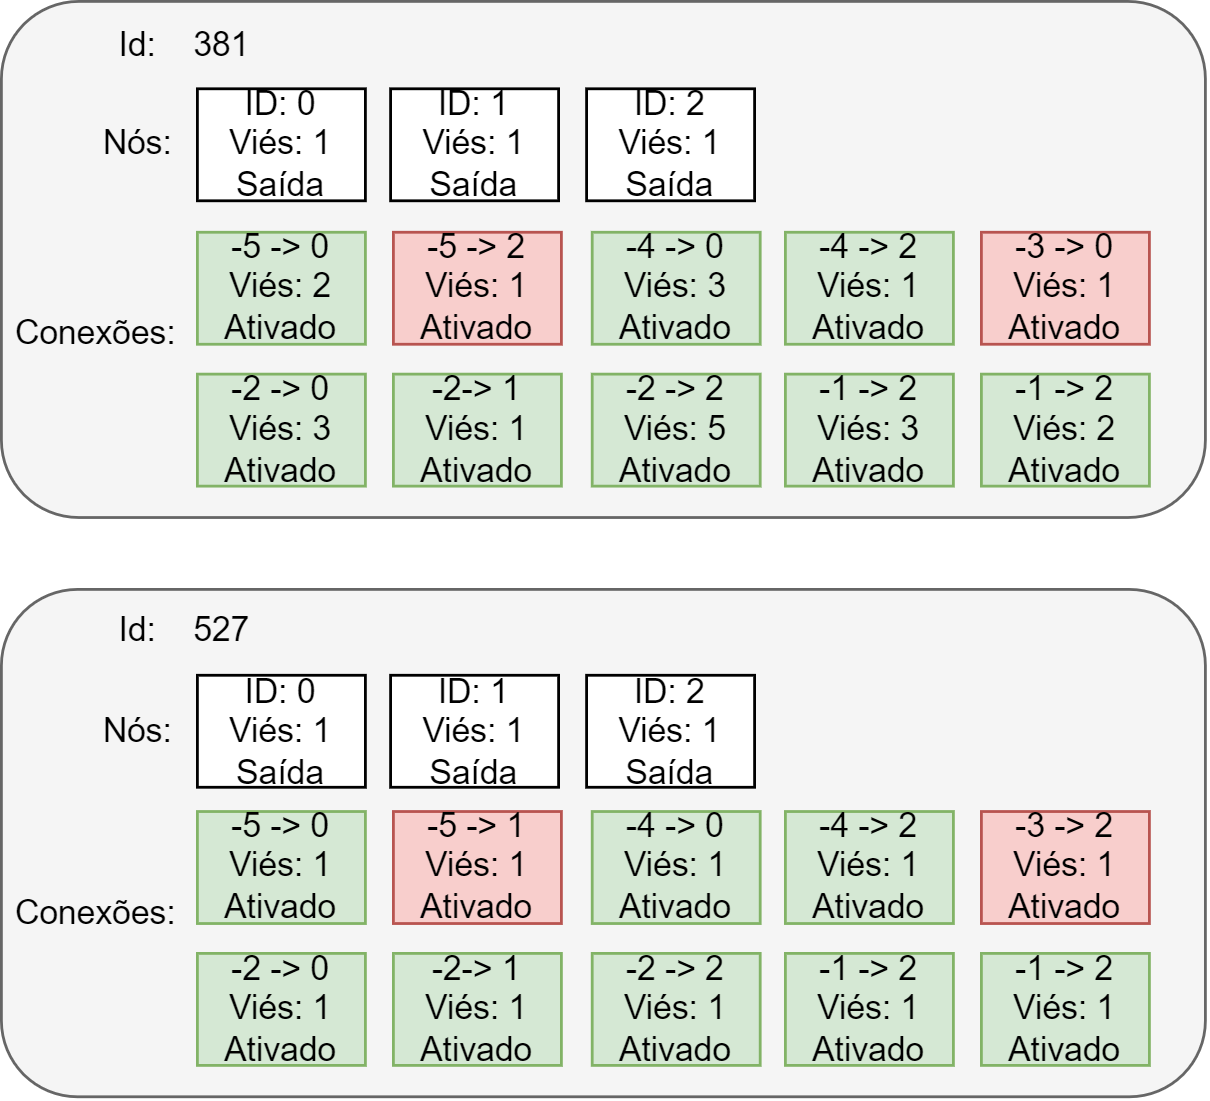
\includegraphics[width=0.7\textwidth]{images/NA.png}
        \legend{
                Fonte: Autoria Pr{\'o}pria.
        }
\end{figure}

Aplicando a fórmula apresentada, o valor 2 (dois) é atribuído à quantidade de nós não correspondentes (em vermelho), enquanto \textit{\overline{W}} pode ser assinalado como a soma de todas as diferenças entre vieses dos genes (conexões) correspondentes (em verde) dividido pela quantidade de tais genes (oito), resultando em 1,5.

Aplicando um coeficiente de 1 (um) para ambos os pesos, os dois fatores podem ser interpretados como detentores de mesma prioridade. Aplicando à fórmula proposta, obtém-se o resultado o seguinte resultado:

\[ \frac{1 * 2}{10} + 1 * 1,5 = 1,7\]

Este valor resultante é então interpretado pela parametrização como dentro ou fora do limiar mínimo para ser considerado ou não de uma determinada espécie. Caso este se encontre fora dos limites, é comparado a outros genomas da população de modo a encontrar sua espécie, caso não seja correspondente a nenhuma, uma nova espécie é criada com este sendo seu primeiro integrante.

\subsection{Encerramento da Execução}
A execução do algoritmo encontra seu fim no momento em que um carro que ultrapasse o limite mínimo de aptidão predefinida é encontrado. A topologia presente em seu genoma é então retornada, e uma simulação de seu trajeto é reproduzida.

Caso a solução não seja encontrada, uma nova iteração é realizada com a nova geração substituindo a antiga população.
